\ifcompact
\section{Evidence so far}
\label{sec:evidence}

We have run the decomposition on one task family: 582 episodes across sixteen sweeps, one
model family, one kernel. The full record---every result, the nulls, and one
retraction---is Appendix~\ref{app:experiments}.


\begin{figure}[t]
\centering
\definecolor{openarm}{HTML}{2A78D6}
\definecolor{bndarm}{HTML}{C4551F}
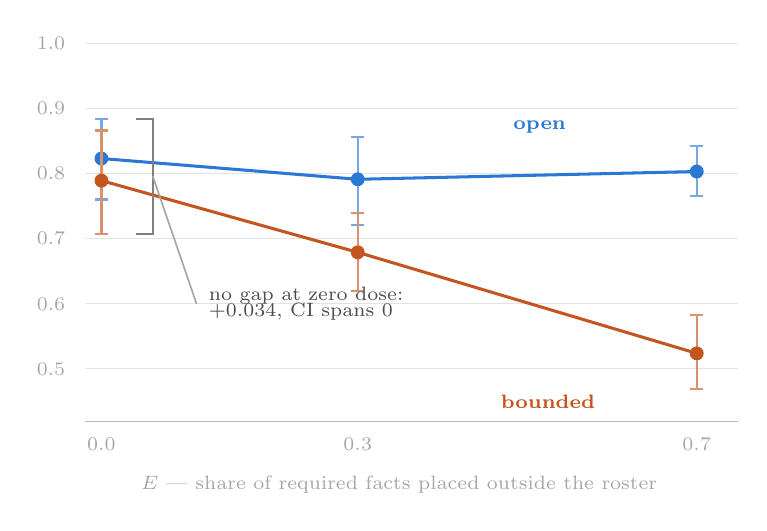
\begin{tikzpicture}[x=1.05cm,y=1.2cm,font=\small]
\draw[gray!22] (-0.2,0.552) -- (7.7,0.552);
\node[anchor=east,gray!70,font=\scriptsize] at (-0.32,0.552) {0.5};
\draw[gray!22] (-0.2,1.241) -- (7.7,1.241);
\node[anchor=east,gray!70,font=\scriptsize] at (-0.32,1.241) {0.6};
\draw[gray!22] (-0.2,1.931) -- (7.7,1.931);
\node[anchor=east,gray!70,font=\scriptsize] at (-0.32,1.931) {0.7};
\draw[gray!22] (-0.2,2.621) -- (7.7,2.621);
\node[anchor=east,gray!70,font=\scriptsize] at (-0.32,2.621) {0.8};
\draw[gray!22] (-0.2,3.310) -- (7.7,3.310);
\node[anchor=east,gray!70,font=\scriptsize] at (-0.32,3.310) {0.9};
\draw[gray!22] (-0.2,4.000) -- (7.7,4.000);
\node[anchor=east,gray!70,font=\scriptsize] at (-0.32,4.000) {1.0};
\draw[gray!55] (-0.2,0.000) -- (7.7,0.000);
\node[anchor=north,gray!70,font=\scriptsize] at (0.00,-0.080) {$0.0$};
\node[anchor=north,gray!70,font=\scriptsize] at (3.10,-0.080) {$0.3$};
\node[anchor=north,gray!70,font=\scriptsize] at (7.20,-0.080) {$0.7$};
\draw[openarm,line width=1.1pt] (0.00,2.779) -- (3.10,2.559) -- (7.20,2.641);
\draw[openarm!65,line width=.8pt] (0.00,2.345) -- (0.00,3.200);
\draw[openarm!65,line width=.8pt] (-0.08,2.345) -- (0.08,2.345);
\draw[openarm!65,line width=.8pt] (-0.08,3.200) -- (0.08,3.200);
\filldraw[openarm] (0.00,2.779) circle (2.3pt);
\draw[openarm!65,line width=.8pt] (3.10,2.076) -- (3.10,3.007);
\draw[openarm!65,line width=.8pt] (3.02,2.076) -- (3.18,2.076);
\draw[openarm!65,line width=.8pt] (3.02,3.007) -- (3.18,3.007);
\filldraw[openarm] (3.10,2.559) circle (2.3pt);
\draw[openarm!65,line width=.8pt] (7.20,2.386) -- (7.20,2.910);
\draw[openarm!65,line width=.8pt] (7.12,2.386) -- (7.28,2.386);
\draw[openarm!65,line width=.8pt] (7.12,2.910) -- (7.28,2.910);
\filldraw[openarm] (7.20,2.641) circle (2.3pt);
\draw[bndarm,line width=1.1pt] (0.00,2.545) -- (3.10,1.786) -- (7.20,0.717);
\draw[bndarm!65,line width=.8pt] (0.00,1.979) -- (0.00,3.076);
\draw[bndarm!65,line width=.8pt] (-0.08,1.979) -- (0.08,1.979);
\draw[bndarm!65,line width=.8pt] (-0.08,3.076) -- (0.08,3.076);
\filldraw[bndarm] (0.00,2.545) circle (2.3pt);
\draw[bndarm!65,line width=.8pt] (3.10,1.379) -- (3.10,2.200);
\draw[bndarm!65,line width=.8pt] (3.02,1.379) -- (3.18,1.379);
\draw[bndarm!65,line width=.8pt] (3.02,2.200) -- (3.18,2.200);
\filldraw[bndarm] (3.10,1.786) circle (2.3pt);
\draw[bndarm!65,line width=.8pt] (7.20,0.338) -- (7.20,1.124);
\draw[bndarm!65,line width=.8pt] (7.12,0.338) -- (7.28,0.338);
\draw[bndarm!65,line width=.8pt] (7.12,1.124) -- (7.28,1.124);
\filldraw[bndarm] (7.20,0.717) circle (2.3pt);
\node[openarm,anchor=south,font=\scriptsize\bfseries] at (5.3,2.941) {open};
\node[bndarm,anchor=north,font=\scriptsize\bfseries] at (5.4,0.377) {bounded};
\draw[black!50,line width=.7pt] (0.42,3.200) -- (0.62,3.200) -- (0.62,1.979) -- (0.42,1.979);
\draw[black!35,line width=.6pt] (0.62,2.593) -- (1.15,1.241);
\node[black!70,font=\scriptsize,align=left,anchor=west] at (1.18,1.241) {no gap at zero dose:\\[-2pt]$+0.034$, CI spans $0$};
\node[anchor=north,gray!70,font=\scriptsize] at (3.6,-0.480) {$E$ --- share of required facts placed outside the roster};
\end{tikzpicture}
\caption{The formation effect is reach, and the dose-response says so. \metric{E} is the
share of a task's required facts placed outside the roster; bars are 95\% percentile
bootstrap intervals over episodes. Four things hold at once, and the axis needs all four:
the contrast \textbf{vanishes at zero dose}, which is the control it had to pass; the arm
that cannot be affected is \textbf{flat} across all three doses; the mechanism variable
tracks the dose (the bounded arm's useful sources fall $4.36 \to 3.17 \to 1.26$); and
fabrication appears only as sources dry up ($0 \to 0.139 \to 0.333$ per task).}
\label{fig:dose}
\end{figure}


\begin{center}\small
\begin{tabular}{@{}p{0.28\linewidth}p{0.64\linewidth}@{}}
\toprule
\textbf{Finding} & \textbf{Evidence} \\
\midrule
Only formation is an intervention
& The two diagonals of one factorial give $0.181$ and $0.314$ on the same episodes; the
  factorial recovers $0.248$ formation and $0.066$ semantics (CI $[+0.012,+0.119]$, $+19$k
  tokens), and $\approx\!0$ attributes. 56 contrasts per beat against a chance floor of
  $2.8$; the two that cleared reverse sign between beats of the same episodes; a
  length-matched placebo of two neutral lines moves the score $+0.005$. \\
\addlinespace[2pt]
The formation effect is reach
& Dose-response in \metric{E} (Figure~\ref{fig:dose}): $+0.034$ (CI $[-0.067,+0.137]$) at
  $E=0$, $+0.111$ at $0.3$, $+0.279$ at $0.7$. The public arm is flat across all three
  doses; the private arm's useful sources fall $4.36 \to 3.17 \to 1.26$. \\
\addlinespace[2pt]
A roster sees less bad information and believes more of it
& Shown a third as much planted misinformation; writes $0.269$ against $0.094$ instances
  per task into the deliverable ($+0.175$, CI $[+0.105,+0.242]$). Across 287 and 286
  delivered tasks the public arms fabricated once, the private arms 58 times. Matching on
  sources obtained does not close it (2.4\% against 18.1\% at four sources). \\
\addlinespace[2pt]
An introduction does work an endorsement does not
& One brokered hop recovers $+0.140$ (CI $[+0.073,+0.204]$) of a $0.304$ gap, replicating
  within three edge-cost strata, and cuts fabrication $0.223 \to 0.057$. Read-all with deep
  ties only inside the roster is indistinguishable from full openness ($+0.019$). Both are
  formation manipulations; every attribute manipulation is flat. \\
\addlinespace[2pt]
\textbf{The bounded arm is weakly dominated}
& It never scores higher, and it spends $\sim$19k more tokens per task at every $E$
  including $E=0$, where its roster holds everything the task needs and it ties on accuracy.
  Its one better column---1.7 fewer counterparts disclosed to---appears only at $E=0.7$,
  where it also scores $0.279$ lower and fabricates in a third of its tasks. \\
\bottomrule
\end{tabular}
\end{center}

\paragraph{So if a private agent network is worth building, our measurements do not contain
the reason.} Three candidates sit outside the scorer. \emph{Confidentiality}: our only proxy
is how many counterparts learn the goal, and it favours the bounded arm only where that arm
has failed. \emph{Recourse}: accountability needs a second encounter, and every episode here
is a cold start (\S\ref{sec:lifecycle}). \emph{Adversaries}: 36 of 100 cards carry plausible
tags and no knowledge, but every agent that is asked answers honestly. What the data does
rule out is the justification most often given---that a bounded network produces better
information. It produces worse information, more expensively. Two limits are ours rather
than the framework's: one model family carries every sweep with a live main effect, and the
scenario predictions of \S\ref{sec:combination} are predictions.
\else
\section{Evidence so far}
\label{sec:evidence}

We have run the decomposition on one task family: 582 episodes across sixteen sweeps, one
model family, one kernel. The full inventory, every result including the nulls and one
retraction, is Appendix~\ref{app:experiments}. Five findings bear on the framework.

\paragraph{Only formation is an intervention.} A naive public-versus-private contrast
returns $0.181$ or $0.314$ on requirement $F_1$ depending on which pairing is called public
and which private---the two diagonals of one factorial, on one set of episodes. The
factorial recovers what neither diagonal isolates: $0.248$ (CI $[+0.194, +0.302]$) from edge
formation, $0.066$ (CI $[+0.012, +0.119]$, and 19k tokens a task) from edge semantics, and
nothing distinguishable from zero on attributes. That axis was tested across 56 contrasts
per beat against a chance floor of $2.8$; two cleared and reversed sign between beats of the
same episodes, and a length-matched placebo of two neutral lines moved the score by
$+0.005$. Prior trust and attribution, the two properties deployed reputation systems carry,
are the flattest measurements in the set.


\begin{figure}[t]
\centering
\definecolor{openarm}{HTML}{2A78D6}
\definecolor{bndarm}{HTML}{C4551F}
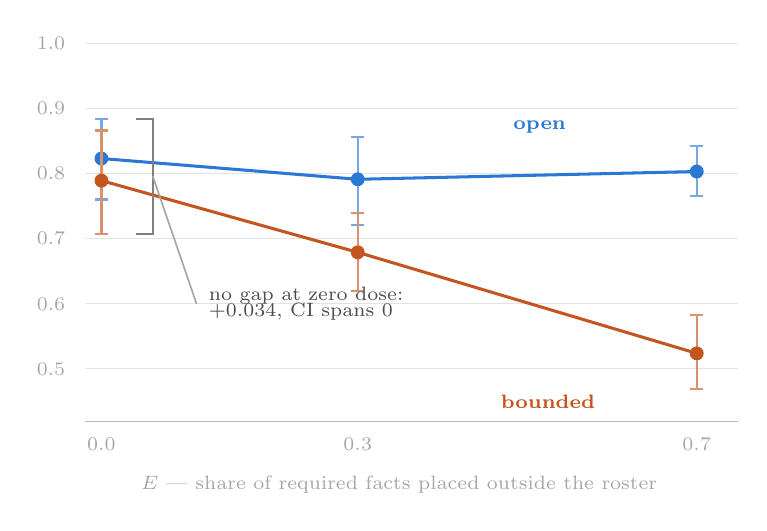
\begin{tikzpicture}[x=1.05cm,y=1.2cm,font=\small]
\draw[gray!22] (-0.2,0.552) -- (7.7,0.552);
\node[anchor=east,gray!70,font=\scriptsize] at (-0.32,0.552) {0.5};
\draw[gray!22] (-0.2,1.241) -- (7.7,1.241);
\node[anchor=east,gray!70,font=\scriptsize] at (-0.32,1.241) {0.6};
\draw[gray!22] (-0.2,1.931) -- (7.7,1.931);
\node[anchor=east,gray!70,font=\scriptsize] at (-0.32,1.931) {0.7};
\draw[gray!22] (-0.2,2.621) -- (7.7,2.621);
\node[anchor=east,gray!70,font=\scriptsize] at (-0.32,2.621) {0.8};
\draw[gray!22] (-0.2,3.310) -- (7.7,3.310);
\node[anchor=east,gray!70,font=\scriptsize] at (-0.32,3.310) {0.9};
\draw[gray!22] (-0.2,4.000) -- (7.7,4.000);
\node[anchor=east,gray!70,font=\scriptsize] at (-0.32,4.000) {1.0};
\draw[gray!55] (-0.2,0.000) -- (7.7,0.000);
\node[anchor=north,gray!70,font=\scriptsize] at (0.00,-0.080) {$0.0$};
\node[anchor=north,gray!70,font=\scriptsize] at (3.10,-0.080) {$0.3$};
\node[anchor=north,gray!70,font=\scriptsize] at (7.20,-0.080) {$0.7$};
\draw[openarm,line width=1.1pt] (0.00,2.779) -- (3.10,2.559) -- (7.20,2.641);
\draw[openarm!65,line width=.8pt] (0.00,2.345) -- (0.00,3.200);
\draw[openarm!65,line width=.8pt] (-0.08,2.345) -- (0.08,2.345);
\draw[openarm!65,line width=.8pt] (-0.08,3.200) -- (0.08,3.200);
\filldraw[openarm] (0.00,2.779) circle (2.3pt);
\draw[openarm!65,line width=.8pt] (3.10,2.076) -- (3.10,3.007);
\draw[openarm!65,line width=.8pt] (3.02,2.076) -- (3.18,2.076);
\draw[openarm!65,line width=.8pt] (3.02,3.007) -- (3.18,3.007);
\filldraw[openarm] (3.10,2.559) circle (2.3pt);
\draw[openarm!65,line width=.8pt] (7.20,2.386) -- (7.20,2.910);
\draw[openarm!65,line width=.8pt] (7.12,2.386) -- (7.28,2.386);
\draw[openarm!65,line width=.8pt] (7.12,2.910) -- (7.28,2.910);
\filldraw[openarm] (7.20,2.641) circle (2.3pt);
\draw[bndarm,line width=1.1pt] (0.00,2.545) -- (3.10,1.786) -- (7.20,0.717);
\draw[bndarm!65,line width=.8pt] (0.00,1.979) -- (0.00,3.076);
\draw[bndarm!65,line width=.8pt] (-0.08,1.979) -- (0.08,1.979);
\draw[bndarm!65,line width=.8pt] (-0.08,3.076) -- (0.08,3.076);
\filldraw[bndarm] (0.00,2.545) circle (2.3pt);
\draw[bndarm!65,line width=.8pt] (3.10,1.379) -- (3.10,2.200);
\draw[bndarm!65,line width=.8pt] (3.02,1.379) -- (3.18,1.379);
\draw[bndarm!65,line width=.8pt] (3.02,2.200) -- (3.18,2.200);
\filldraw[bndarm] (3.10,1.786) circle (2.3pt);
\draw[bndarm!65,line width=.8pt] (7.20,0.338) -- (7.20,1.124);
\draw[bndarm!65,line width=.8pt] (7.12,0.338) -- (7.28,0.338);
\draw[bndarm!65,line width=.8pt] (7.12,1.124) -- (7.28,1.124);
\filldraw[bndarm] (7.20,0.717) circle (2.3pt);
\node[openarm,anchor=south,font=\scriptsize\bfseries] at (5.3,2.941) {open};
\node[bndarm,anchor=north,font=\scriptsize\bfseries] at (5.4,0.377) {bounded};
\draw[black!50,line width=.7pt] (0.42,3.200) -- (0.62,3.200) -- (0.62,1.979) -- (0.42,1.979);
\draw[black!35,line width=.6pt] (0.62,2.593) -- (1.15,1.241);
\node[black!70,font=\scriptsize,align=left,anchor=west] at (1.18,1.241) {no gap at zero dose:\\[-2pt]$+0.034$, CI spans $0$};
\node[anchor=north,gray!70,font=\scriptsize] at (3.6,-0.480) {$E$ --- share of required facts placed outside the roster};
\end{tikzpicture}
\caption{The formation effect is reach, and the dose-response says so. \metric{E} is the
share of a task's required facts placed outside the roster; bars are 95\% percentile
bootstrap intervals over episodes. Four things hold at once, and the axis needs all four:
the contrast \textbf{vanishes at zero dose}, which is the control it had to pass; the arm
that cannot be affected is \textbf{flat} across all three doses; the mechanism variable
tracks the dose (the bounded arm's useful sources fall $4.36 \to 3.17 \to 1.26$); and
fabrication appears only as sources dry up ($0 \to 0.139 \to 0.333$ per task).}
\label{fig:dose}
\end{figure}


\paragraph{The formation effect is reach, and the dose-response says so.} With
\metric{E}---the share of required facts outside the roster---as the dose, the contrast runs
$+0.034$ (95\% CI $[-0.067, +0.137]$, spans zero) at $E=0$ (Figure~\ref{fig:dose}), $+0.111$
at $E = 0.3$ and $+0.279$ at $E = 0.7$. The zero-dose cell is the control the axis had to
pass and did: a private network that can already reach what a task needs is not worse. The
public arm is flat across all three doses ($0.823 / 0.791 / 0.803$), so the manipulation is
specific to the arm it should affect, and the mechanism variable tracks it---the private
arm's useful sources fall $4.36 \to 3.17 \to 1.26$.

\paragraph{A roster sees less bad information and believes more of it.} This is the one
result we did not design (Figure~\ref{fig:credulity}, in the appendix). The private arm is shown roughly a
quarter as much planted misinformation as the public arm, and writes it into the deliverable
\emph{more}---$0.269$ against $0.094$ instances per task (difference $+0.175$, CI
$[+0.105, +0.242]$). When it reaches no one at all it does not decline to answer: across
matched sets of 287 and 286 delivered tasks, the public arms fabricated a value once and the
private arms 58 times. Filtering misinformation out before it arrives also removes the
second source that would have caught it, which is the redundancy argument of
\S\ref{sec:framework} appearing as a failure mode rather than as a benefit. That explanation
is not the whole mechanism, and we say so because the tidier version is available and wrong:
among beats that obtained four useful sources the absorption rate is 2.4\% open against
18.1\% bounded, so starvation amplifies credulity without being all of it.

\ifcompact\else
\begin{figure}[t]
\centering
\definecolor{openarm}{HTML}{2A78D6}
\definecolor{bndarm}{HTML}{C4551F}
\definecolor{brokerc}{HTML}{9A7A3E}
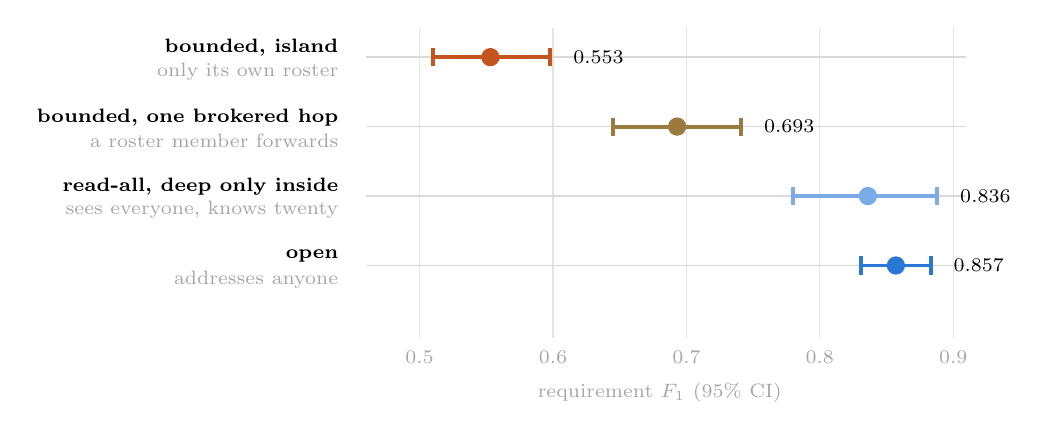
\begin{tikzpicture}[x=1.05cm,y=1.05cm,font=\small]
\draw[gray!22] (0.645,-0.30) -- (0.645,3.45);
\node[gray!70,font=\scriptsize,anchor=north] at (0.645,-0.34) {0.5};
\draw[gray!22] (2.259,-0.30) -- (2.259,3.45);
\node[gray!70,font=\scriptsize,anchor=north] at (2.259,-0.34) {0.6};
\draw[gray!22] (3.873,-0.30) -- (3.873,3.45);
\node[gray!70,font=\scriptsize,anchor=north] at (3.873,-0.34) {0.7};
\draw[gray!22] (5.486,-0.30) -- (5.486,3.45);
\node[gray!70,font=\scriptsize,anchor=north] at (5.486,-0.34) {0.8};
\draw[gray!22] (7.100,-0.30) -- (7.100,3.45);
\node[gray!70,font=\scriptsize,anchor=north] at (7.100,-0.34) {0.9};
\draw[gray!30,line width=.5pt] (0,3.10) -- (7.25,3.10);
\draw[bndarm,line width=1.4pt] (0.807,3.10) -- (2.227,3.10);
\draw[bndarm,line width=1.4pt] (0.807,2.99) -- (0.807,3.21);
\draw[bndarm,line width=1.4pt] (2.227,2.99) -- (2.227,3.21);
\filldraw[bndarm] (1.501,3.10) circle (3.1pt);
\node[font=\scriptsize,anchor=west] at (2.387,3.10) {0.553};
\node[font=\scriptsize\bfseries,anchor=east,align=right] at (-0.22,3.21) {bounded, island};
\node[font=\scriptsize,gray!70,anchor=east,align=right] at (-0.22,2.93) {only its own roster};
\draw[gray!30,line width=.5pt] (0,2.26) -- (7.25,2.26);
\draw[brokerc,line width=1.4pt] (2.985,2.26) -- (4.534,2.26);
\draw[brokerc,line width=1.4pt] (2.985,2.15) -- (2.985,2.37);
\draw[brokerc,line width=1.4pt] (4.534,2.15) -- (4.534,2.37);
\filldraw[brokerc] (3.760,2.26) circle (3.1pt);
\node[font=\scriptsize,anchor=west] at (4.694,2.26) {0.693};
\node[font=\scriptsize\bfseries,anchor=east,align=right] at (-0.22,2.37) {bounded, one brokered hop};
\node[font=\scriptsize,gray!70,anchor=east,align=right] at (-0.22,2.09) {a roster member forwards};
\draw[gray!30,line width=.5pt] (0,1.42) -- (7.25,1.42);
\draw[openarm!62,line width=1.4pt] (5.164,1.42) -- (6.906,1.42);
\draw[openarm!62,line width=1.4pt] (5.164,1.31) -- (5.164,1.53);
\draw[openarm!62,line width=1.4pt] (6.906,1.31) -- (6.906,1.53);
\filldraw[openarm!62] (6.067,1.42) circle (3.1pt);
\node[font=\scriptsize,anchor=west] at (7.066,1.42) {0.836};
\node[font=\scriptsize\bfseries,anchor=east,align=right] at (-0.22,1.53) {read-all, deep only inside};
\node[font=\scriptsize,gray!70,anchor=east,align=right] at (-0.22,1.25) {sees everyone, knows twenty};
\draw[gray!30,line width=.5pt] (0,0.58) -- (7.25,0.58);
\draw[openarm,line width=1.4pt] (5.987,0.58) -- (6.826,0.58);
\draw[openarm,line width=1.4pt] (5.987,0.47) -- (5.987,0.69);
\draw[openarm,line width=1.4pt] (6.826,0.47) -- (6.826,0.69);
\filldraw[openarm] (6.406,0.58) circle (3.1pt);
\node[font=\scriptsize,anchor=west] at (6.986,0.58) {0.857};
\node[font=\scriptsize\bfseries,anchor=east,align=right] at (-0.22,0.69) {open};
\node[font=\scriptsize,gray!70,anchor=east,align=right] at (-0.22,0.41) {addresses anyone};
\node[gray!70,font=\scriptsize,anchor=north] at (3.550,-0.72) {requirement $F_1$ (95\% CI)};
\end{tikzpicture}
\caption{An introduction does work an endorsement does not. All four rows are formation
manipulations, and every one of them moves; every \txt{attribute} manipulation---including
the ones asserting exactly the trust a broker would carry---is flat. One brokered hop
recovers $+0.140$ (CI $[+0.073, +0.204]$) of the $0.304$ gap and cuts fabrication from
$0.223$ to $0.057$ per task; letting a bounded arm read the whole directory while keeping
deep relationships inside the roster is indistinguishable from full openness ($+0.019$,
spans zero). Depth of relationship is not what is bought here---a second reachable source
is.}
\label{fig:ladder}
\end{figure}
\fi

\paragraph{An introduction does work an endorsement does not.} A bounded roster given a
single brokered hop---one roster member may forward a request to a counterpart the requester
cannot address---recovers close to half the gap to the open arm, and most of the fabrication
with it; letting a bounded arm \emph{read} the whole directory while keeping deep
relationships inside the roster is indistinguishable from full openness
(Figure~\ref{fig:ladder}). Both are formation manipulations, and both move. Every attribute
manipulation is flat, including the ones asserting exactly the trust an introduction would
carry. This is the endorsement/introduction distinction of \S\ref{sec:framework} landing
where the framework said it would: what changes the graph does work, what describes it does
not.

\paragraph{On everything we measured, the bounded arm is weakly dominated.} The
decomposition invites a symmetric reading that the data does not support, so this is worth
stating without hedging.

\begin{center}\small
\begin{tabular}{@{}lrrr@{}}
\toprule
\textbf{bounded $-$ open} & \textbf{$E=0$} & \textbf{$E=0.3$} & \textbf{$E=0.7$} \\
\midrule
requirement $F_1$         & tie              & $-0.111^\ast$      & $-0.279^\ast$ \\
tokens per task           & $+18.8$k$^\ast$  & $+19.5$k$^\ast$    & $+19.1$k$^\ast$ \\
wall clock                & tie              & $+0.8$\,min$^\ast$ & $+0.5$\,min$^\ast$ \\
fabrications per task     & tie (both $0$)   & $+0.139^\ast$      & $+0.319^\ast$ \\
counterparts disclosed to & tie              & tie                & $-1.7^\ast$ \\
\bottomrule
\end{tabular}\\[1pt]
{\footnotesize $^\ast$ 95\% CI excludes zero.}
\end{center}

\noindent The $E=0$ column is the private network's best case: its roster already holds
every fact the task needs. It does not win there. It ties on accuracy and spends 38\% more
tokens to do it---an overhead of $+17.9$k in one harness generation and $+19.3$k in the
other, so not an artifact of either. Its growth is explained (the bounded arm searches its
twenty-card roster $6.8 \to 10.1 \to 16.2$ times as $E$ rises while its useful sources fall,
which is what looking harder for something that is not there costs); the baseline at $E=0$
is not. The one column where it looks better is disclosure, and only at $E=0.7$, where it
also scores $0.279$ lower and fabricates in a third of its tasks. \textbf{A network that
leaks less because it reached nobody has not protected anything.}

\paragraph{So if a private agent network is worth building, our measurements do not contain
the reason.} Three candidates sit outside the scorer, and each names its own experiment.
\emph{Confidentiality}: our only proxy is how many counterparts learn the goal, and it
favours the bounded arm only where that arm has failed---a real test needs a disclosure term
in the objective, not a by-product of contact count. \emph{Recourse}: accountability needs a
second encounter to mean anything, and every episode here is a cold start
(\S\ref{sec:lifecycle}). \emph{Adversaries}: 36 of 100 cards carry plausible tags and no
knowledge, but every agent that is asked answers honestly, so the defence a private network
exists to provide has nothing to defend against here. What the data does rule out is the
justification most often given: that a bounded network produces better information. It
produces worse information, more expensively.

Two further limits are ours rather than the framework's. One model family carries every
sweep with a live main effect---the second-model replication was run only at $E=0$, the
control cell, so model-independence is not established. And the scenario predictions of
\S\ref{sec:combination} are predictions.
\fi
